\documentclass[thesis]{subfiles}

\begin{document}

\chapter{Protokół komunikacji}

Głównym celem niniejszej pracy jest opracowanie i~implementacja protokołu komunikacji serwera i~klienta tak, aby~serwer mógł wydajnie i~bezpiecznie przekazać klientom \emph{co},~a~nie \emph{jak}, mają zmienić w~swojej konfiguracji, aby~dostosować się do~wymagań postawionych przez administratora sieci komputerowej. Tak~przedstawiony cel może nasunąć na~myśl pomysł wykorzystania bezpołączeniowego protokołu opartego na~\hrefemph{https://en.wikipedia.org/wiki/IP_multicast}{multicastowym} rozsyłaniu konfiguracji klientów przez serwer. Należy jednak pamiętać, że~warstwą transportową dla~metod multicastowych jest protokół~\href{https://en.wikipedia.org/wiki/User_Datagram_Protocol}{UDP}, który z~zasady działania jest zawodny, tzn.~nie gwarantuje, że~pakiety nie zostaną zduplikowane i~że~każdy wysłany pakiet dotrze do~celu, a~jeśli nawet dotrze, to~niekoniecznie w~takiej kolejności w~jakiej był wysłany. Ponadto protokół~UDP nie uwzględnia m.in.~kontroli przepływu, tzn.~w~szczególności pakiety mogą przychodzić do~odbiorcy szybciej niż~ten może je~przetworzyć.

Naturalną alternatywą dla~UDP jest~TCP, jednak TCP, w~porównaniu do~UDP, jest złożonym protokołem połączeniowym wartswy transportowej, w~ramach którego przesyła się~wiele dodatkowych metadanych gwarantujących niezawodność połączenia, której nie zapewnia~UDP. Rozsyłanie przez serwer tej samej konfiguracji dużej liczbie klientów korzystając z~TCP wiązałoby się~z~nawiązywaniem połączenia z~każdym z~nich z~osobna, co~wydaje się być zbędne i~w~konsekwencji nieoptymalne~(por.~rys.~\ref{fig:unicast-vs-multicast}).

\begin{figure}
	\centering
	\includegraphics[width=0.8\textwidth]{img/unicast-vs-multicast}
	\caption{Zobrazowanie porównania unicastu i~multicastu\\(rys.~ze~strony projektu~\href{http://zeromq.org/}{ØMQ}~na~licencji \glslink{copyleft}{copyleft} \href{https://creativecommons.org/licenses/by-sa/3.0/}{CC~BY-SA~3.0})}
	\label{fig:unicast-vs-multicast}
\end{figure}

Kompromisem mógłby okazać się alternatywny protokół warstwy transportowej. Jednym z~przykładów takiego protokołu jest~\href{https://en.wikipedia.org/wiki/QUIC}{QUIC}~(\emph{Quick UDP Internet Connections}) opracowany przez Google i~stosowany domyślnie w~przeglądarce internetowej \hrefemph{https://www.google.pl/chrome/}{Chrome} do~nawiązywania połączeń ze~stronami internetowymi obsługiwanymi przez serwery Google. Celem projektowym QUIC było zminimalizowanie opóźnień w~protokole~TCP, upodabniając go~do UDP, jednocześnie zachowując zalety TCP i~dodając bezpieczeństwo połączenia oparte na~protokole~\gls{ssl/tls}~\cite{quic-wire-layout-spec,quic-crypto,quic-roskind}. W~czasie pisania tej~pracy QUIC nie jest jeszcze ustandaryzowany przez~\gls{ietf}, chociaż w~2016~roku powstał zespół, który pracuje nad~jego standaryzacją~\cite{quic-draft,quic-workinggroup}.

Innym przykładem alternatywnego protokołu warstwy transportowej jest~\href{https://en.wikipedia.org/wiki/Pragmatic_General_Multicast}{PGM}~(\emph{Pragmatic General Multicast}), który został zaprojektowany przez firmę \hrefemph{http://www.cisco.com/}{Cisco} z~myślą o~aplikacjach z~względnie prostymi wymaganiami dotyczącymi niezawodności, korzystających z~potencjału multicastingu~\cite{pgm-rfc}. Założenia projektowe~PGM zostały przedstawione w~\href{https://tools.ietf.org/html/rfc3208}{RFC3208} i~są~bardzo bliskie potrzebom projektowanego protokołu, dlatego warstwą transportową projektowanego rozwiązania jest~PGM zaimplementowany w~ramach projektu \hrefemph{https://code.google.com/archive/p/openpgm/}{OpenPGM} i~wykorzystany w~bibliotece \hrefemph{http://zeromq.org/}{ZeroMQ}. % Przy tej okazji warto wspomnieć, że~w~IPv6 wycofano \emph{broadcast} na~rzecz multicastingu.

%Motywacją dlaOpracowany protokół komunikacji opiera się na~protokole~TCP. Bezpieczeństwo protokołu zapewnia wykorzystanie biblioteki OpenSSL, która implementuje protokół~SSL/TLS. Oba te~elementy, tzn.~opracowany protokół aplikacji oraz~wykorzystana biblioteka OpenSSL, działają w~warstwie aplikacji modelu~\gls{tcpip}.
%
%W~niniejszym rozdziale opisano architekturę i~aspekty bezpieczeństwa protokołu.

%------------------------------------------------------------------------------

\section{Protokół PGM}

Protokół \href{https://tools.ietf.org/html/rfc3208}{PGM}~(\emph{Pragmatic General Multicast}, a~pierwotnie \emph{Pretty Good Multicasting}) to~protokół do~rozgłaszania pakietów, korzystający z~multicastingu, dzięki czemu wystarczy, że~w~czasie danej sesji rozgłoszeniowej, serwer wyśle tylko raz to, co ma do~zakomunikowania swoim klientom. Powielenie wiadomości do~wszystkich klientów, którzy zgłosili chęć otrzymywania multicastu odbywa się na~poziomie działania \emph{routera}, do~którego klient jest podłączony bezpośrednio lub pośrednio, tzn.~np.~za~pomocą przełączników sieciowych~(\emph{switchy}). Dołączenie i~opuszczenie grupy multicastowej przez klienta odbywa się w~sieciach IPv4 dzięki~protokołowi warstwy sieciowej \href{https://en.wikipedia.org/wiki/Internet_Group_Management_Protocol}{IGMP}~(\emph{Internet Group Management Protocol}), a~w~sieciach IPv6 dzięki protokołowi~\href{https://en.wikipedia.org/wiki/Multicast_Listener_Discovery}{MLD}~(\emph{Multicast Listener Discovery}) wbudowanemu w~protokół \href{https://en.wikipedia.org/wiki/Internet_Control_Message_Protocol_version_6}{ICMPv6}~(\emph{Internet Control Message Protocol version~6}). Protokół IGMP~istnieje w~trzech wersjach: IGMPv1, IGMPv2, IGMPv3 opisanych odpowiednio w:~\href{https://tools.ietf.org/html/rfc1112}{RFC1112}, \href{https://tools.ietf.org/html/rfc2236}{RFC2236} i~\href{https://tools.ietf.org/html/rfc3376}{RFC3376} (zaktualizowany przez~\href{https://tools.ietf.org/html/rfc4604}{RFC4604}). Protokół MLD~został opisany~w~\href{https://tools.ietf.org/html/rfc3810}{RFC3810} i~został zaktualizowany w~\href{https://tools.ietf.org/html/rfc4604}{RFC4604}.

Protokół~PGM różni się od~zwykłego multicastingu opartego na~protokole~UDP m.in.~tym, że~pakiety zostają oznaczone sekwencyjnie liczbami całkowitymi, dzięki czemu klienci są~w~stanie stwierdzić czy~jakieś pakiety zostały ,,zgubione''. Jeśli klient wykryje, że~nie otrzymał wszystkich pakietów, ma~możliwość przez pewien, z~góry zdefiniowany czas\footnote{Ściśle rzecz biorąc okno czasowe (\emph{Transmit Window}) w~ramach którego klient może poprosić o~retransmisję pakietów, może być zdefiniowane za~pomocą czasu, liczby bajtów lub~liczby pakietów.}, wysłać prośbę o~retransmisję zadanych pakietów. W~przeciwieństwie do~protokołu UDP, PGM~gwarantuje, że~klient albo odbierze wszystkie pakiety i~ich ewentualne retransmisje, albo wykryje nieodwracalną utratę pakietów.

W~PGM każde źródło multicastingu ma~przydzielony unikalny identyfikator TSI~(\emph{Transport Session Identifier}) będący wynikiem konkatenacji identyfikatora~GSI\footnote{\href{https://tools.ietf.org/html/rfc3208\#page-33}{RFC3208~zaleca}, aby~za~GSI przyjąć wartość funkcji haszującej~\href{https://en.wikipedia.org/wiki/MD5}{MD5} dla~48~najmłodszych (najmniej znaczących) bitów sygnatury~DNS serwera.}~(\emph{Global Source~ID}) oraz~portu używanego przez serwer. Podczas normalnego działania protokołu PGM, serwer wysyła multicastem dane do~klientów w~pakietach \texttt{ODATA}\footnote{Nazwa pakietu \texttt{ODATA} i~inne nazwy pakietów PGM przywołane w~tym rozdziale pochodzą z~\href{https://tools.ietf.org/html/rfc3208}{RFC3208}, definiującego protokół~PGM.} (\emph{Original Data}), a~klienci, jeśli wykryją brakujące pakiety, wysyłają unicastem do~ostatniego routera na drodze od~serwera do~klienta, pakiet \texttt{NAK}~(\emph{Negative Acknowledgment}) tak długo, jak długo nie otrzymają w~odpowiedzi pakietu \texttt{NCF}~(\emph{NAK Confirmation}). Serwer numeruje kolejnymi liczbami całkowitymi (cyklicznie) z~zakresu~$[0,~2^{32}-1]$ każdy kolejny pakiet \texttt{ODATA} z~danymi przekazanymi przez warstwę aplikacji. Router który otrzyma pakiet \texttt{NAK} przekazuje go do~routera poziom wyżej lub, jeśli router jest podłączony bezpośrednio do~serwera, przekazuje \texttt{NAK} serwerowi. Na~każdym poziomie przekazywania \texttt{NAK} w~górę drzewa, którego korzeniem jest serwer, zostaje rozesłany multicastem pakiet \texttt{NCF} tylko na~interfejsie, na~którym przyszedł pakiet~\texttt{NAK}. Pakiety \texttt{NAK} pokonują dokładnie tą~samą drogę co~dane \texttt{ODATA}, tylko od~końca, co~jest ważne dla~przesyłanych pakietów naprawczych \texttt{RDATA}~(\emph{Repair Data}), ponieważ routery otrzymując~\texttt{NAK} zapamiętują m.in.~to, że~otrzymały taki pakiet i~numer interfejsu na~którym go~otrzymały, ustanawiając stan naprawczy~(\emph{Repair State}). Jeśli pakiet naprawczy \texttt{RDATA} zostałby wysłany do~routera, który nie ma ustawionego stanu naprawczego zostałby zignorowany. Pomiędzy pakietami \texttt{ODATA} są~co~jakiś czas przesyłane pakiety SPM~(\emph{Source Path Messages}), dzięki którym pakiety \texttt{NAK} wracają dokładnie tą~ścieżką od~klienta do~serwera, którą został wysłany pakiet \texttt{ODATA}. W~szczególności dzięki~SPM klient wie który router jest ostatni na~drodze od~źródła do~niego semgo i~do~tego właśnie routera kieruje unicastem pakiety~\texttt{NAK}. ,,Zgubione'' pakiety są~retransmitowane w~odpowiedzi na~pakiety \texttt{NAK} pakietami \texttt{RDATA} przez serwer lub~tzw.~DLR~(\emph{Designated Local Repairer}), którym może być któryś z~klientów. PGM~specyfikuje mechanizmy minimalizacji przekazywanych duplikatów \texttt{NAK}~w~górę drzewa oraz procedurę, dzięki której pakiety naprawcze \texttt{RDATA} nie są~przekazywane do~tych części sieci, z~których nie były wysyłane pakiety~\texttt{NAK}. PGM~może bez utraty funkcjonalności (ale~z~częściową stratą wydajności --- chyba, że~wszyscy klienci i~serwer są~podpięci do~jednego routera) działać w~sieciach, w~których część lub~żaden router nie implementuje tego protokołu.

Warto zauważyć, że~w~tak zaprojektowanym protokole, w~przeciwieństwie np.~do~protokołu~TCP, nie ma pakietów~\texttt{ACK}, które potwierdzałyby odbiór pakietów \texttt{ODATA} przez klientów. Dzięki temu zyskujemy niezawodność multicastingu, jednocześnie nie tracąc jego zalet jakimi są~szybkość i~skalowalność.

%Multicast jest stosunkowo rzadko używany wśród aplikacji, częściej jest używany w~protokołach routingu i~niskopoziomowych protokołach do~odkrywania topologii sieci.

%------------------------------------------------------------------------------

\section{Architektura protokołu}

Zaprojektowany protokół działa w~modelu klient-serwer. Serwer spełnia rolę nadzorcy nad~oprogramowaniem i~konfiguracją klientów. Specyfikacja konfiguracji klientów oraz lista klientów zarządzanych przez serwer jest przechowywana w~plikach tekstowych zapisanych na~serwerze w~formacie \hreftt{https://en.wikipedia.org/wiki/YAML}{YAML}\footnote{Wybór tego formatu plików konfiguracyjnych jest podyktowany czytelnością plików zapisanych w~tym formacie.}. Serwer nie utrzymuje żadnego rejestru ani~bazy danych faktycznego stanu oprogramowania zainstalowanego na~maszynach klientów. Rolą serwera, podobnie jak we~wszystkich rozwiązaniach przedstawionych w~rozdziale~\ref{sec:istniejace-rozwiazania}, jest przechowywanie czytelnych dla~człowieka plików tekstowych, opisujących oczekiwany stan konfiguracji klientów, który jest niezależny od~konfiguracji i~dystrybucji \glslink{gnulinux}{Linux} klientów. Dodatkową, drugorzędną rolą serwera jest logowanie ewentualnych niepowodzeń dostosowywania się klientów do~wymagań serwera.

W~uproszczeniu działanie protokołu sprowadza się do~okresowego\footnote{Okres ten jest konfigurowalny za~pomocą pliku konfiguracyjnego serwera.} rozgłaszania konfiguracji klientów multicastem za~pomocą protokołu~PGM, zapewniającym komunikację niezawodną, uporządkowaną i~pozbawioną duplikatów pakietów. Niezawodność PGM~należy rozumieć w~ten sposób, że~PGM gwarantuje, że~odbiorca multicastingu odbierze wszystkie rozgłoszone pakiety lub~wykryje nieodwracalną utratę pakietów, których nie~można już retransmitować w~danej sesji, co~wiąże się z~zasadą działania protokołu~PGM, który utrzymuje okno czasowe, w~którym znajdują się~pakiety, które nadawca musi być w~stanie retransmitować jeśli okaże się, że~któryś z~odbiorców wyśle pakiet~\texttt{NAK}~(\emph{Negative Acknowledgment}). Tak~rozesłana konfiguracja jest zapisana w~formacie, który nie jest uzależniony od~żadnej konkretnej dystrybucji \glslink{gnulinux}{Linux} --- zawiera ona~m.in.:
\begin{itemize}
	\item informację o~tym jakie pakiety oprogramowania powinny być:
	\begin{itemize}
		\item zainstalowane na~maszynie klienta,
		\item odinstalowane na~maszynie klienta,
	\end{itemize}
	w~tym w~szczególności informacja o~nazwie i~wersji pakietu oprogramowania.
	\item opcjonalne pliki konfiguracyjne dostarczone przez administratora, nadpisujące domyślną konfigurację wybranych paczek oprogramowania.
\end{itemize}

Przez określenie \emph{pakiet oprogramowania} należy rozumieć oficjalne, dostarczone przez opiekunów danej dystrybucji \glslink{gnulinux}{Linux}, skompresowane pliki instalacyjne programów, zarządzane przez menadżer pakietów. W~kontekście implementacji dostarczonej w~ramach niniejszej pracy są~to pakiety oprogramowania formatu~\hreftt{https://en.wikipedia.org/wiki/Deb_(file_format)}{deb} i~\hreftt{https://en.wikipedia.org/wiki/Tar_(computing)}{tar.xz} oraz odpowiadające im~menadżery pakietów \hreftt{https://www.debian.org/doc/manuals/apt-guide/ch2.html}{apt-get}\footnote{Na~systemie \emph{Debian} zazwyczaj korzysta się z~\texttt{apt-get} lub~\texttt{aptitude}, które korzysta z~właściwego, niskopoziomowego menadżera pakietów \hreftt{https://en.wikipedia.org/wiki/Dpkg}{dpkg}.} i~\hreftt{https://www.archlinux.org/pacman/pacman.8.html}{pacman} pochodzące odpowiednio z~systemu operacyjnego \hrefemph{https://en.wikipedia.org/wiki/Debian}{Linux~Debian} i~\hrefemph{https://en.wikipedia.org/wiki/Arch_Linux}{Linux~Arch}.

Każdy klient serwera jest przyporządkowany do~pewnej niepustej grupy komputerów, które otrzymają tą~samą konfigurację z~serwera, dlatego zanim klient ją~otrzyma, musi zadeklarować do~której grupy chce należeć. W~tym celu klient, korzystając z~protokołu \emph{IGMP}, wysyła pakiet \emph{join} z~ustawionym polem \texttt{IP} na~wybrany adres multicastowy serwera, który odpowiada wybranej grupie. Adres ten jest ustawiany przez administratora sieci w~konfiguracji serwera i~klienta. Opcjonalnie, w~konfiguracji serwera można włączyć multicastowe rozgłaszanie listy wszystkich obsługiwanych multicastowych adresów~IP i~odpowiadających im~nazwy ustalone przez administratora, dzięki czemu aplikacja klienta jest zdolna wyświetlić wszystkie adresy multicastowe\footnote{Zakres adresów multicastowych jest regulowany przez \gls{iana}. Zakres adresów~IP na~potrzeby multicastu: 224.0.0.0 -- 239.255.255.255, przy czym adresy z~zakresu 224.0.0.0 -- 224.0.0.255 \href{https://www.iana.org/assignments/multicast-addresses/multicast-addresses.xhtml}{są}~wykorzystywane m.in.~przez protoły trasowania oraz protokoły wykrywające topologię sieci i~nie są~wykorzystywane przez aplikacje~(patrz: \href{https://tools.ietf.org/html/rfc5771}{5771}).}, na~których rozgłaszane są~konfiguracje klientów. Przykładowo taką listą (zapisaną w~notacji \emph{Pythonowej}) może być:
\begin{lstlisting}[numbers=none,frame=none]
[
	[ { 'name' : 'Laboratorium 301' }, { 'IP' : '224.100.100.100' } ],
	[ { 'name' : 'Biblioteka'       }, { 'IP' : '224.100.100.200' } ]
]
\end{lstlisting}

 wysyła pakiet \emph{IGMP} nie powiadamiając bezpośrednio serwer o~wyborze. Warto zauważyć, że~mając $n$~klientów podzielonych na~$k$~grup multicastowych, którym odpowiadają konkretne zestawy konfiguracji klientów, serwer wysyła tylko $k$, a~nie~$n\cdot k$ wiadomości. Jest to~możliwe dzięki przerzuceniu odpowiedzialności zduplikowania wiadomości na~\emph{router(y)}. Takie podejście przyczynia się do~obniżenia obciążenia sieci i~w~konsekwencji polepsza skalowalność protokołu.

przed otrzymaniem konfiguracji od~serwera klient musi zadeklarować ednak zanim klient otrzyma multicastem konfigurację od~serwera, musi TODO TODO TODO

Początek działania klienta rozpoczyna się od~zgłoszenia chęci otrzymywania multicastingu na~adresie~IP ustalonym po~stronie serwera. Początkowo klient nie należy do~żadnej grupy multicastowej.

Każda grupa multicastowa reprezentuje pewien zestaw oprogramowania i~konfiguracji. Każdy klient może należeć do~jednej lub~kilku grup multicastowych. Za~zapisanie się do~grupy odpowiada protokół~\href{https://en.wikipedia.org/wiki/Internet_Group_Management_Protocol}{IGMP}.

%------------------------------------------------------------------------------

\section{Bezpieczeństwo protokołu}
\label{sec:security}

Uwzględnienie bezpieczeństwa protokołu jest krytyczne dla~powodzenia projektu protokołu, szczególnie takiego, który umożliwia serwerowi na~zarządzanie konfiguracją dziesiątek, setek lub~tysięcy klientów. Zaniedbanie bezpieczeństwa protokołu lub~jego wadliwa implementacja, umożliwiłaby atakującemu system, na~przejęcie kontroli nad~wszystkimi klientami, np.~przez przesłanie klientom złośliwych aktualizacji oprogramowania lub~konfiguracji.

Umożliwienie przejęcia kontroli nad~wszystkimi klientami byłoby prawdopodobnie najgorszym z~możliwych scenariuszy zarówno dla użytkowników jak i~administratora atakowanej sieci, jednak niedbała implementacja protokołu mogłaby umożliwiać również wiele innych rodzajów ataków, np.~\emph{replay attack} i~\emph{man in the middle~(MITM)}. W~celu uniknięcia podatności protokołu na~wymienione i~inne, popularne rodzaje ataków, należy zagwarantować bezpieczeństwo protokołu co~najmniej pod~względem:
\begin{enumerate}
\item uwierzytelnienia co~najmniej serwera,
\item poufności komunikacji,
\item integralności komunikacji.
\end{enumerate}
W~celu maksymalnego zaostrzenia rygorów bezpieczeństwa protokołu, do~powyższych własności można dodać również inne, w~szczególności, własność \emph{\glslink{pfs}{Perfect Forward Secrecy~(PFS)}} (patrz rozdział~\ref{subsec:pfs}).

W~kolejnych podrozdziałach zostaną opisane metody, które zostały wykorzystane do~zapewnienia poszczególnych elementów, składających się na~bezpieczeństwo protokołu. Wszystkie opisane dalej algorytmy i~metody kryptograficzne zostały wykorzystane przez niniejszy projekt przez wykorzystanie popularnej, otwartoźródłowej biblioteki kryptograficznej~\gls{openssl}, implementującej protokół kryptograficzny~\gls{ssl/tls}.

%---------------------------------------

\subsection{SSL/TLS}
\label{subsec:ssl-tls}

Protokół \gls{ssl/tls} jest bardzo elastyczny pod~względem doboru algorytmów i~metod kryptograficznych. Elastyczność objawia się nie tylko możliwością skonfigurowania konkretnych algorytmów, które posłużą do~zapewnienia uwierzytelnienia, poufności, integralności komunikacji i~ustalenia klucza sesji, ale również możliwością zdefiniowania za~pomocą słów kluczowych, zbioru algorytmów spośród których serwer i~klient, podczas negocjacji w~ramach \emph{handshake'u} sesji \gls{ssl/tls}, wybierają jeden, najsilniejszy z~tych, które wspierają.

Przykładowo, jeśli celem jest dopuszczenie do~użytku wyłącznie zestawów metod kryptograficznych używających algorytmu \glslink{dh}{Diffiego-Hellmana} do~wymiany klucza, a~do szyfrowania szyfru blokowego~\gls{aes}, to~filtr będzie miał postać napisu \texttt{DH+AES @STRENGTH}. Słowo kluczowe \texttt{@STRENGTH} służy do~posortowania wynikowych zestawów metod kryptograficznych nierosnąco (a~nie ściśle malejąco) względem bezpieczeństwa.

Aby przekonać się jakie algorytmy zostaną zwrócone dla danego filtru, nie~trzeba korzystać z~API biblioteki \gls{openssl}. Wystarczy nam do~tego konsola, co~prezentuje listing~\ref{lst:openssl-console-filter}.\\

\begin{lstlisting}[numbers=none,language=bash,caption={Wynik filtrowania zestawów algorytmów w~konsoli za~pomocą \gls{openssl}},label=lst:openssl-console-filter]
$ openssl ciphers -v 'DH+AES @STRENGTH'
AES256-GCM-SHA384   TLSv1.2 Kx=RSA  Au=RSA  Enc=AESGCM(256)  Mac=AEAD
AES256-SHA256       TLSv1.2 Kx=RSA  Au=RSA  Enc=AES(256)     Mac=SHA256
AES256-SHA          SSLv3 Kx=RSA    Au=RSA  Enc=AES(256)     Mac=SHA1
AES128-GCM-SHA256   TLSv1.2 Kx=RSA  Au=RSA  Enc=AESGCM(128)  Mac=AEAD
AES128-SHA256       TLSv1.2 Kx=RSA  Au=RSA  Enc=AES(128)     Mac=SHA256
AES128-SHA          SSLv3 Kx=RSA    Au=RSA  Enc=AES(128)     Mac=SHA1
\end{lstlisting}

Filtr złożony ze~słów kluczowych, wykorzystany w~implementacji projektu zarówno dla serwera, jak i~klienta, został przedstawiony na listingu~\ref{lst:openssl-filter}. Filtr ten jest bardzo restrykcyjny, tak, aby zapewnić~\gls{pfs}. Wykrzyknik w~filtrze pełni rolę operatora logicznego~\texttt{not}.\\

\begin{lstlisting}[numbers=none,caption={Filtr \gls{openssl} dla algorytmów użytych w~projekcie},label=lst:openssl-filter]
kEECDH+ECDSA kEECDH kEDH +SHA !aNULL !eNULL !LOW !3DES !MD5 !EXP !DSS !PSK !SRP !kECDH !CAMELLIA !IDEA !RC4 !SEED @STRENGTH
\end{lstlisting}

Pełny opis słów kluczowych można znaleźć w~dokumentacji \gls{openssl} oraz~w~darmowej, regularnie aktualizowanej elektronicznej książce\footnote{Jest ona częścią większej książki pt.~,,Bulletproof SSL and TLS"~(ISBN:~978-1907117046). Projekt \gls{openssl} ma~raczej opinię słabo udokumentowanego, dlatego te~książki mają spore znaczenie praktyczne.} pt.~,,OpenSSL Cookbook'' autorstwa Ivana Ristić'a, polecanej na~oficjalnej stronie internetowej projektu~\gls{openssl}~\cite{openssl-cookbook-suites}.

%---------------------------------------

\subsection{Uwierzytelnienie}

Uwierzytelnienie serwera przez klienta jest krytyczne dla~bezpieczeństwa protokołu. Gdyby nie ono, to~atakujący mógłby podawać się za~serwer i~przesłać klientowi dowolną konfigurację i~oprogramowanie. Gdyby komunikacja była szyfrowana, ale nieuwierzytelniona, to~atakujący mógłby również podjąć próby ataku \emph{replay attack}. W~celu uniknięcia tego problemu wykorzystano certyfikat X.509 dla~serwera~\cite{wiki:x509}.

Wygenerowanie takiego certyfikatu wymaga podpisania przez centrum certyfikacji~(\gls{ca})~\cite{wiki:ca}. Ze~względu na~brak potrzeby posiadania w~trakcie implementacji certyfikatu podpisanego przez uznane \gls{ca}, a~także ze~względu na~względnie duże koszty finansowe i~czasowe z~tym związane, w~czasie implementacji wykorzystano certyfikat podpisany przez siebie~(ang.~\emph{self-signed certificate}). Konfiguracja klienta pozwala w~trybie \texttt{debug} zaufać takiemu certyfikatowi. Oczywiście, w~przypadku wdrożenia projektu, należałoby postarać się o~certyfikat podpisany przez uznany~\gls{ca}.

Wygenerowanie i~podpisanie certyfikatu zostało wykonane z~użyciem \gls{openssl}. Listing~\ref{lst:openssl-gencert} przedstawia jak wygenerować klucze publiczny i~prywatny \gls{rsa} o~długości 4096~bitów, a~następnie, jak wykorzystać klucz prywatny do~wygenerowania żądania podpisania certyfikatu (ang.~\emph{Certificate signing request}) i~na jego podstawie podpisać certyfikat~X.509~\cite{openssl-cookbook,wiki:csr}.

\begin{lstlisting}[numbers=none,caption={Wygenerowanie i~podpisanie certyfikatu X.509},label=lst:openssl-gencert]
$ openssl genrsa -aes256 -out rsa_aes256_4096.key 4096
$ openssl req -new -key rsa_aes256_4096.key -out request.csr
$ openssl req -new -config request.cnf -key fd.key -out request.csr
$ openssl x509 -req -days 365 -in request.csr -signkey rsa_aes256_4096.key -out certificate.pem
\end{lstlisting}

Przykładowa zawartość pliku \path{request.cnf}, który służy do~konfiguracji żądania podpisania certyfikatu przedstawia listing~\ref{lst:openssl-request-config}.

\begin{lstlisting}[numbers=none,caption={Plik z~konfiguracją certyfikatu X.509},label=lst:openssl-request-config]
[req]
default_bits       = 4096
default_keyfile    = rsa_aes256_4096.key
prompt             = no
distinguished_name = dn
req_extensions     = ext
input_password     = minipw

[dn]
CN                 = Patryk
OU                 = MiNI
emailAddress       = patryk.beza@gmail.com
O                  = PW
L                  = Warsaw
ST                 = Masovian
C                  = PL

[ext]
subjectAltName     = DNS:www.mini.pw.edu.pl,DNS:*.mini.pw.edu.pl
\end{lstlisting}

Aby sprawdzić czy~certyfikat jest przez nas zaufany, wystarczy wydać komendę:
\begin{lstlisting}[numbers=none]
$ openssl verify -verbose certificate.pem
\end{lstlisting}

%---------------------------------------

\subsection{Poufność}

Poufność komunikacji nie jest tak krytyczna jak uwierzytelnienie serwera, jednak jest również istotna, ponieważ atakujący podsłuchujący komunikację między serwerem i~klientami, mógłby się~wiele dowiedzieć o~wersjach i~konfiguracji oprogramowania klientów. Dzięki zdobytej wiedzy, atakujący mógłby przeanalizować np.~czy oprogramowanie klientów jest przestarzałe i~podatne na~ataki, czy konfiguracja oprogramowania pozwala na~wykorzystanie luk bezpieczeństwa.

Komunikacja między serwerem i~klientem jest szyfrowana symetrycznym, blokowym szyfrem \gls{aes} z~kluczem 256-bitowym~(preferowane podczas negocjacji) lub~128-bitowym. Dla~obu długości klucza możliwe jest działanie w~trybie~GCM\footnote{\emph{Galois/Counter Mode}.}~(preferowane) lub~domyślnym.

%---------------------------------------

\subsection{Integralność}

Integralność komunikacji jest konieczna, aby zapobiec atakom typu \emph{man in the middle}, polegającym na~modyfikacji komunikacji między serwerem i~klientem, niezależnie od~tego czy jest ona~szyfrowana czy nie.

Algorytm używany do~sprawdzania integralności wiadomości jest negocjowany tak jak algorytmy używane do~zapewnienia uwierzytelnienia, szyfrowania i~ustalenia wspólnego klucza dla symetrycznego algorytmu szyfrującego komunikację (patrz rozdział~\ref{subsec:ssl-tls}). Możliwe algorytmy to: \emph{AEAD}\footnote{Ściśle rzecz biorąc tryb AEAD~(ang.~\emph{Authenticated Encryption with Associated Data}) jest klasą wiązania bloków zaszyfrowanych w~blokowym algorytmie szyfrującym (ang.~\emph{Block cipher mode of operation}. \gls{aes} pracujący w~trybie GCM należy do~tej klasy, dzięki czemu integralność jest zapewniana ,,przy okazji" szyfrowania komunikacji.}, \emph{SHA384}, \emph{SHA256} i~\emph{SHA1}.

%---------------------------------------

\subsection{Perfect Forward Secrecy}
\label{subsec:pfs}

Własność \emph{\glslink{pfs}{Perfect Forward Secrecy}~(PFS)} umożliwia zachowanie poufności komunikacji nawet jeśli atakujący zapisał całą zaszyfrowaną komunikację między serwerem i~klientem, a~po~jakimś czasie uzyskał klucze prywatne obu stron komunikacji. Własność ta~wiąże się ze~sposobem ustalenia sesyjnego klucza dla~symetrycznego szyfru zapewniającego poufność komunikacji (takiego jak np.~\gls{aes}).

W~uproszczeniu problem polega na tym, że~w~przypadku wykorzystania~\gls{rsa} do~ustalenia klucza sesyjnego dla~symetrycznego algorytmu szyfrującego, strona~A komunikacji, używa klucza publicznego strony~B do~zaszyfrowania losowego klucza sesyjnego\footnote{W~rzeczywistości \emph{Pre-Master Key}, z~którego dopiero jest wyliczany ostateczny klucz sesyjny.}~i wysyła go~do~B. Po~skompromitowaniu klucza prywatnego strony~B, atakujący może odczytać całą komunikację między stronami A~i~B, deszyfrując najpierw klucz sesyjny, a~następnie całą komunikację między serwerem i~klientem.

\gls{pfs} radzi sobie z~tym problemem rezygnując z~przesyłania zaszyfrowanego klucza sesyjnego, wprowadzając zamiast tego efemeryczny algorytm \glslink{dh}{Diffiego-Hellmana} w~postaci klasycznej~(\glslink{dh}{EDH})~i krzywoeliptycznej~(ECDHE)~\cite{mimuw-ssl-w04,openssl-cookbook-suites}. Efemeryczny algorytm \glslink{dh}{Diffiego-Hellmana} różni się od~nieefemerycznego tym, że~w~efemerycznej wersji algorytmu parametry algorytmu nie~są stałe, tzn.~np.~nie są zapisane w~certyfikacie. Wersja krzywoliniowa co~do~pomysłu nie różni się istotnie od~wersji klasycznej, tylko działa na krzywych eliptycznych. Wersja krzywoeliptyczna charakteryzuje się~lepszą wydajnością na~większości procesorów ze~względu na~fakt, że~do zapewnienia takiego samego poziomu bezpieczeństwa jakie gwarantuje~\gls{rsa} z~kluczem o~długości 3072~bitów, potrzeba krzywoeliptycznego odpowiednika o~długości 256~bitów.

Poniżej został przedstawiony schemat przebiegu klasycznego algorytmu \glslink{dh}{Diffiego-Hellmana}.

\begin{enumerate}
\item A i~B uzgadniają skończoną, cykliczną grupę~$G$ rzędu~$p$, gdzie $p$ jest liczbą pierwszą i~generator $g$ tej grupy. Atakujący może znać~$g$ oraz~$p$.
\item A wybiera tajną liczbę całkowitą $1 \leq a < n$ i~wysyła do~B liczbę $A=g^a \pmod{p}$.
\item B wybiera tajną liczbę całkowitą $1 \leq b < n$ i~wysyła do~A liczbę $B=g^b \pmod{p}$.
\item A oblicza $s=B^a \pmod{p}$.
\item B oblicza $s=A^b \pmod{p}$.
\item A i~B współdzielą tajną liczbę~$s$.
\end{enumerate}

Podsłuchujący atakujący, aby~poznać liczbę $s$, musiałby rozwiązać tzw.~problem Diffiego-Hellmana, który jest problemem równie trudnym w~sensie teorii złożoności, jak problem algorytmu dyskretnego. Liczby $a$ i~$b$ są~przed wysłaniem podpisywane kluczem prywatnym w~celu uniknięcia ataku~\emph{man in the middle}.

Ilustracja~\ref{fig:dh} obrazowo przedstawia w~jaki sposób działa algorytm \glslink{dh}{Diffiego-Hellmana}.

\begin{figure}
	\centering
	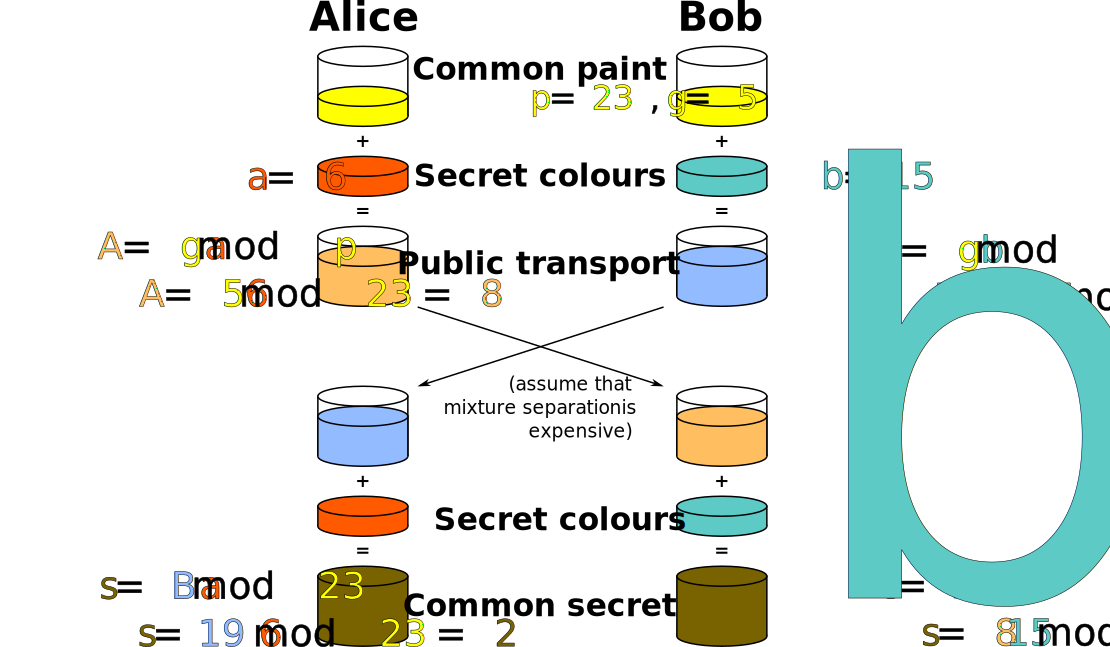
\includegraphics[width=\textwidth]{img/Diffie-Hellman_Key_Exchange_desc}
	\caption{Zobrazowanie działania algorytmu Diffiego-Hellmana (źródło: Wikipedia)}
	\label{fig:dh}
\end{figure}

%---------------------------------------

\subsection{Zestawy kryptograficzne}

W~praktyce, podczas testów, w~czasie których nawiązywano połączenie \gls{ssl/tls} pomiędzy klientem i~serwerem uruchamianym na~systemie z~zainstalowanym \gls{openssl} w~wersji \texttt{1.0.2h}, strony połączenia zawsze negocjowały zestaw algorytmów \texttt{ECDHE-RSA-AES256-GCM-SHA384}, który oznacza użycie najnowszego dostępnej wersji protokołu~\glslink{ssl/tls}{TLS}, tj.~protokołu~TLSv1.2, zapewniającego:
\begin{enumerate}
\item Poufność przez wykorzystanie \gls{aes} pracującym w~trybie GCM z~kluczem o~długości 256~bitów,
\item Ustalenie klucza sesyjnego dla~\gls{aes} przez~wykorzystanie efemerycznej wersji algorytmu \glslink{dh}{Diffiego-Hellmana} w~wersji dla~krzywych eliptycznych~(ECDH),
\item Uwierzytelnienie przez wykorzystanie podpisu cyfrowego z~wykorzystaniem~\gls{rsa},
\item Integralność gwarantowaną przez działanie \gls{aes} w~trybie~GCM. SHA384~w~nazwie wynegocjonowanego zestawu oznacza uczycie funkcji haszującej SHA384 podczas fazy \emph{handshake} i~do rozszerzenia dzielonego sekretu uzyskanego podczas ustalenia klucza~sesyjnego do~klucza symetrycznego dla~\gls{aes}~\cite{stack:openssl-sha-gcm}.
\end{enumerate}

\end{document}
